% v2-acmsmall-sample.tex, dated March 6 2012
% This is a sample file for ACM small trim journals
%
% Compilation using 'acmsmall.cls' - version 1.3 (March 2012), Aptara Inc.
% (c) 2010 Association for Computing Machinery (ACM)
%
% Questions/Suggestions/Feedback should be addressed to => "acmtexsupport@aptaracorp.com".
% Users can also go through the FAQs available on the journal's submission webpage.
%
% Steps to compile: latex, bibtex, latex latex
%
% For tracking purposes => this is v1.3 - March 2012

\documentclass[prodmode,acmtecs]{acmsmall} % Aptara syntax

% Package to generate and customize Algorithm as per ACM style
\usepackage[ruled]{algorithm2e}
\renewcommand{\algorithmcfname}{ALGORITHM}
\SetAlFnt{\small}
\SetAlCapFnt{\small}
\SetAlCapNameFnt{\small}
\SetAlCapHSkip{0pt}
\IncMargin{-\parindent}

\usepackage[nonumberlist]{glossaries}
\setacronymstyle{long-short}
\makenoidxglossaries
% Load acronyms list
\loadglsentries{acronyms}
\usepackage{bm}
\usepackage{prettyref}
\usepackage[T1]{fontenc} % Use 8-bit encoding that has 256 glyphs
\usepackage[utf8]{inputenc} % Required for including letters with accent
\usepackage{graphicx} % Required for including images
\graphicspath{{Figures/}} % Set the default folder for images
\usepackage{enumitem} % Required for manipulating the whitespace between and within lists
\usepackage{lipsum} % Used for inserting dummy 'Lorem ipsum' text into the template
\usepackage{amsmath,amssymb} % For including math equations, theorems, symbols, etc
\usepackage{varioref} % More descriptive referencing
\usepackage{array,multirow}
\allowdisplaybreaks

% Copyright
%\setcopyright{acmcopyright}
%\setcopyright{acmlicensed}
%\setcopyright{rightsretained}
%\setcopyright{usgov}
%\setcopyright{usgovmixed}
%\setcopyright{cagov}
%\setcopyright{cagovmixed}

% Document starts
\begin{document}

% Page heads
\markboth{L. Crestel et P.Esling}{A Conditional model for orchestral Inference}

% Title portion
\title{The Live Orchestral Piano : a conditional model for musical orchestration}
\author{LEOPOLD CRESTEL
\affil{Institut de Recherche et Coordination Acoustique/Musique}
PHILIPPE ESLING
\affil{Institut de Recherche et Coordination Acoustique/Musique}
}
% NOTE! Affiliations placed here should be for the institution where the
%       BULK of the research was done. If the author has gone to a new
%       institution, before publication, the (above) affiliation should NOT be changed.
%       The authors 'current' address may be given in the "Author's addresses:" block (below).
%       So for example, Mr. Abdelzaher, the bulk of the research was done at UIUC, and he is
%       currently affiliated with NASA.

\begin{abstract}
\end{abstract}

% We no longer use \terms command
%\terms{Design, Algorithms, Performance}

\keywords{Automatic orchestration, Conditional Restricted Boltzmann Machine, deep learning}

\acmformat{Léopold Crestel, Philippe Esling, 2010. The Live Orchestral Piano : a conditional model for musical orchestration}
% At a minimum you need to supply the author names, year and a title.
% IMPORTANT:
% Full first names whenever they are known, surname last, followed by a period.
% In the case of two authors, 'and' is placed between them.
% In the case of three or more authors, the serial comma is used, that is, all author names
% except the last one but including the penultimate author's name are followed by a comma,
% and then 'and' is placed before the final author's name.
% If only first and middle initials are known, then each initial
% is followed by a period and they are separated by a space.
% The remaining information (journal title, volume, article number, date, etc.) is 'auto-generated'.

\begin{bottomstuff}
Author's addresses: L. Crestel and P.Esling, Représentation Musicales,
Institut de Recherche et Coordination Acoustique/Musique; 
\end{bottomstuff}

\maketitle

\section{Introduction}
% Orchestration classique
\begin{figure}
\centering
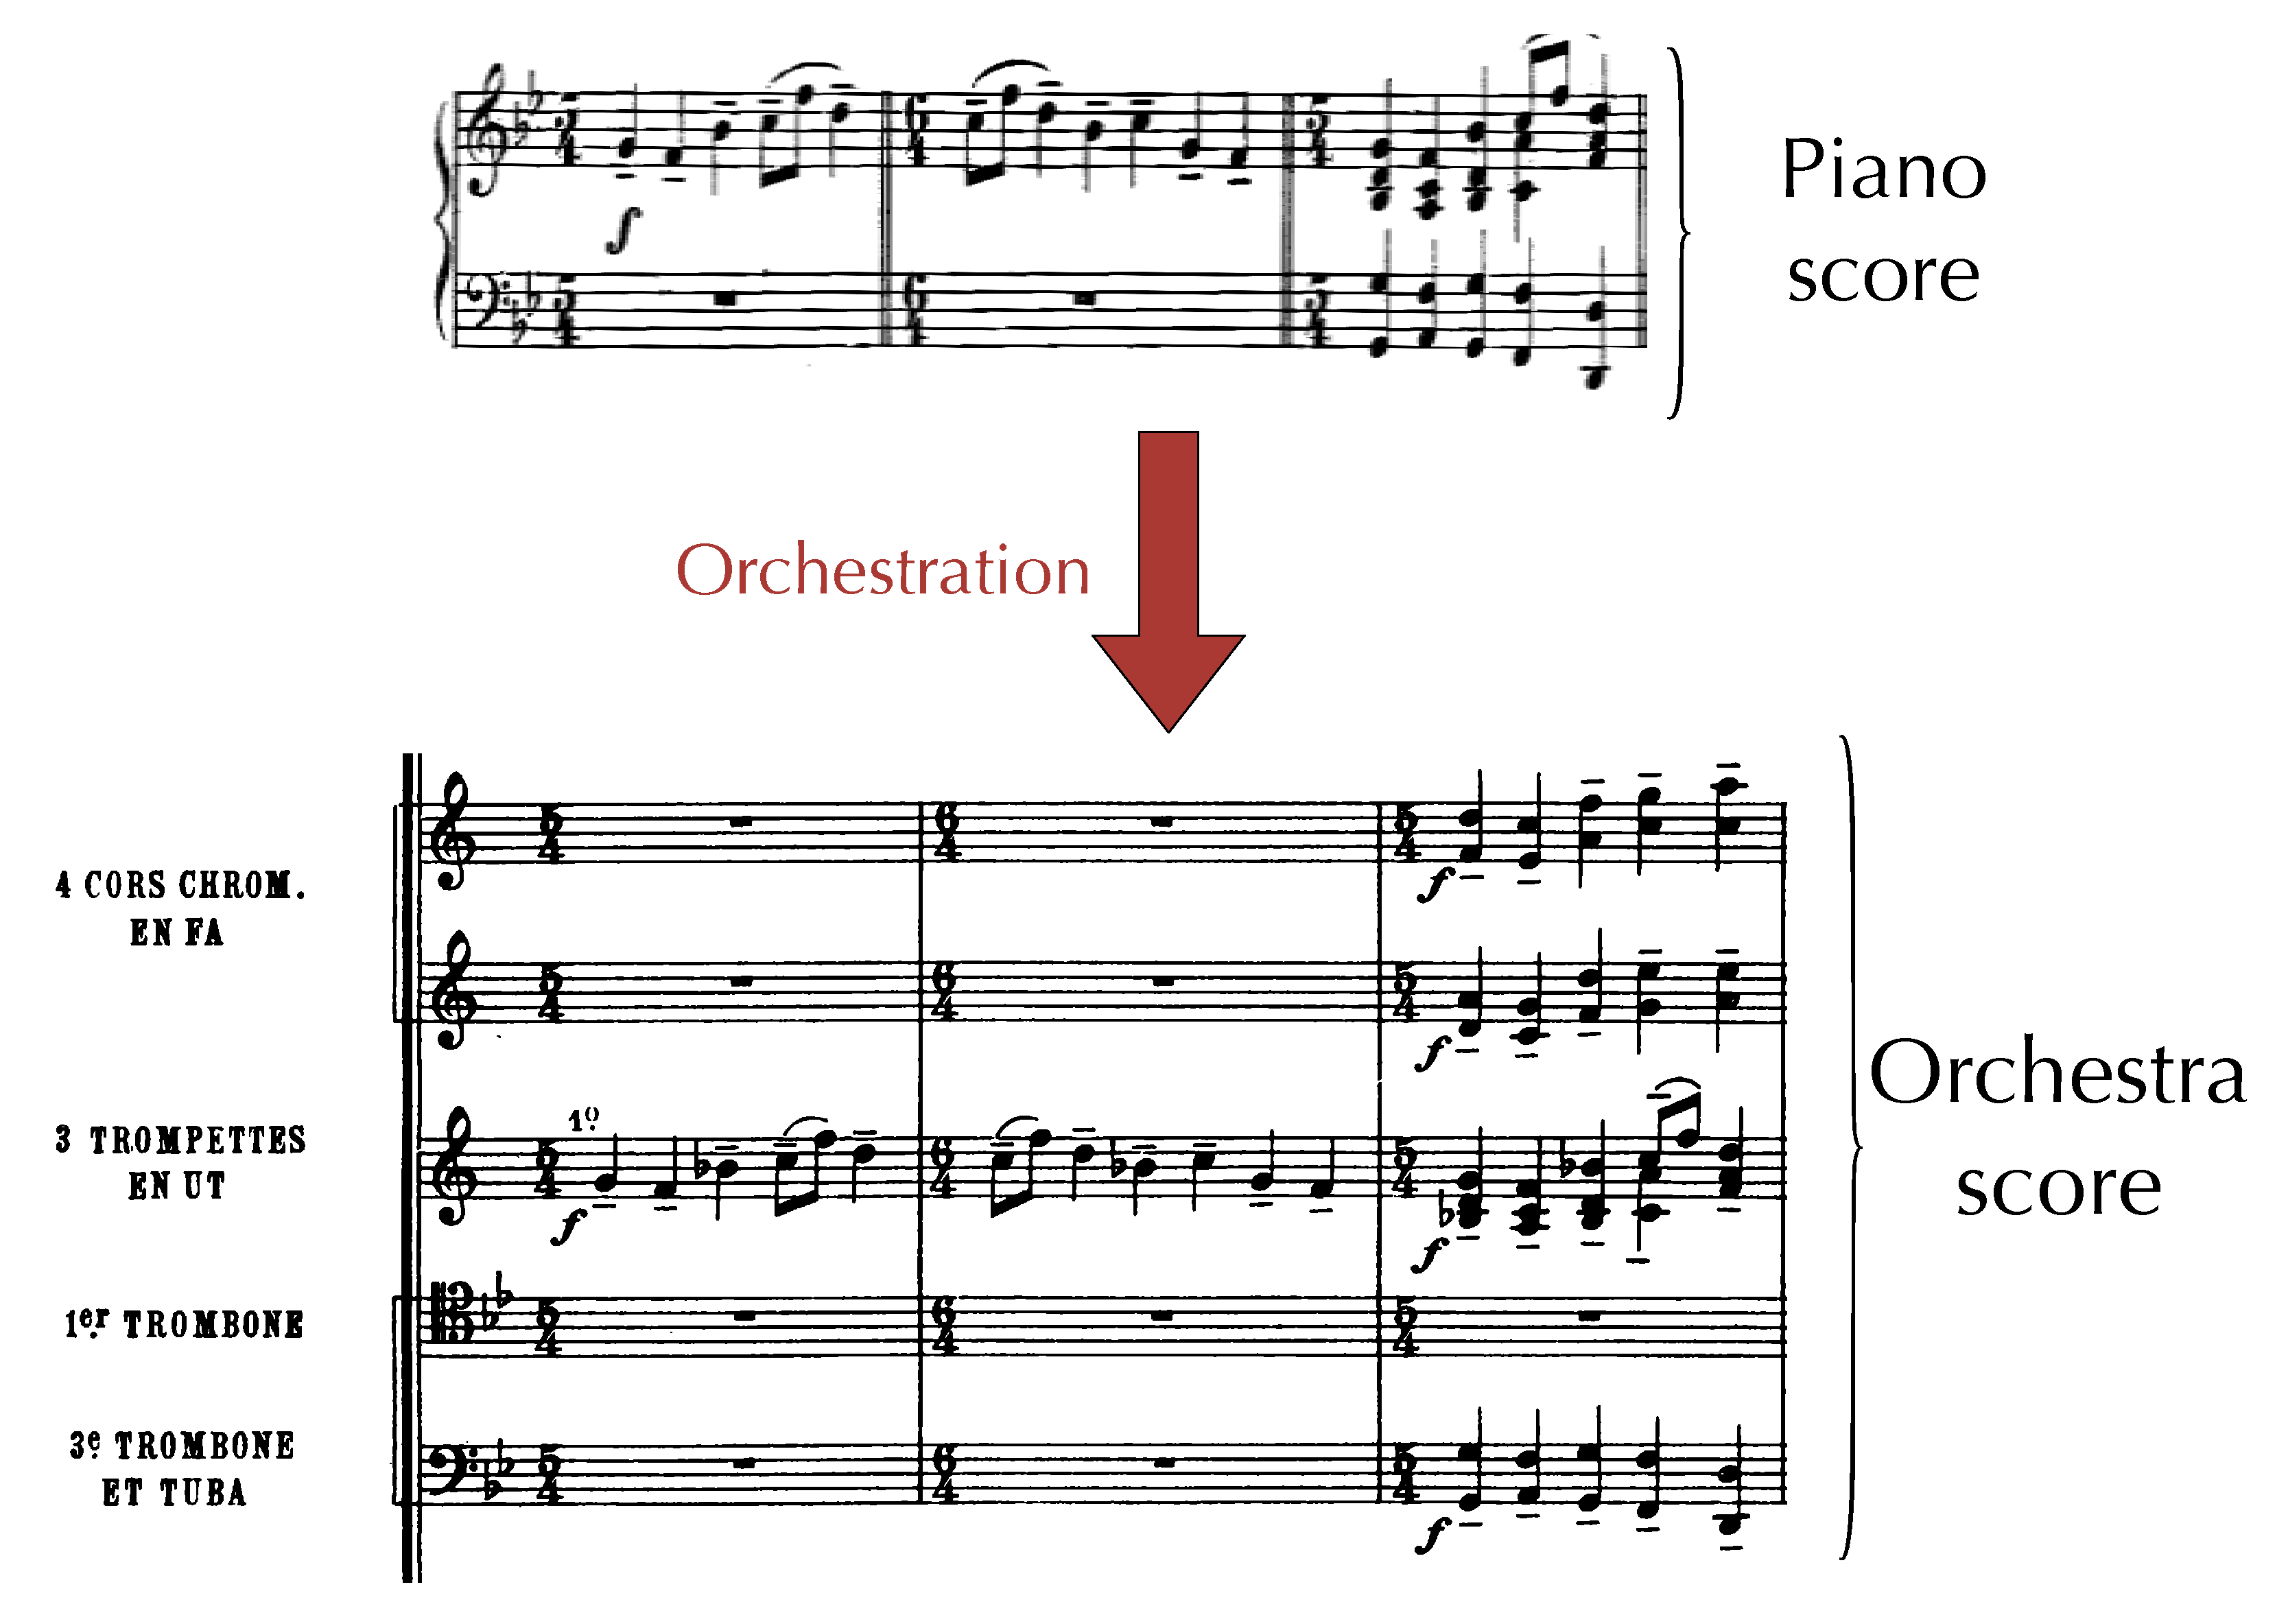
\includegraphics[scale=0.2]{orch}
\label{fig:orch}
\caption{\textit{Projective orchestration}. A piano score is extended (projected) on an orchestra. For one piano score, many acceptable orchestration exist. Our hypothesis is that a piano score is strongly correlated to any of the orchestration that could be produced from this piece.}
\end{figure}
%% Musical orchestration : why is it so hard ?
\textit{Musical orchestration} is the subtle art of writing musical pieces for the orchestra, by combining the spectral properties specific to each instrument in order to achieve a particular sonic goal. This apparently simple definition evokes the tremendous complexity that lies in the transformation from a symbolic representation (the score) to an acoustic rendering (the performance of the piece by an orchestra).
As pointed out by Walter Piston \cite{piston-orch}, the gap between the two is huge, and the musical notation fails at describing most of the important dimensions of an orchestral work (timbre, couleurs, REFERENCE BLENDING et effets orchestraux). An immediate observation is the versatility of the different interpretations of the same written piece. A more embarrassing consequence is the fact that orchestration remains a mainly empirical discipline, learned through the observation of orchestrations from the elder \cite{berlioz_orch,koechli_orch}, but not axiomatized in books.
Behind the lack of theoretic construction shines the huge complexity of the discipline.
Indeed, if we solely consider the range of notes, dynamics, chords and playing modes provided by a single musical instrument, we can foresee the infinite number of combinations provided by the many instrument that form an orchestra. This huge combinatorial problem is complicated by the non-linear behaviour of instrument mixtures' spectral properties. Computer-aided orchestration aims at designing tools to help composers exploring the massive sets of instrumental possibilities, discover new kind of solutions and formalize unexplained mechanisms in order to build a theory of orchestration.

%% Projective and injective. SOA automatic injective orchestration
The wide definition we gave of orchestration actually covers many different sub-problems from which arise two different paradigms for writing orchestral music. Among those, we can distinguish \textit{injective} and \textit{projective} orchestration \cite{eslingthesis}. The \textit{injective} paradigm was born from the problem of finding the best instrument in order to reconstruct a particular sound. A typical question would be which instrument and how should the play in order to recreate the sound of a crying baby. A more abstract and general point of view is to define a timbre target that should be matched with an instrumental mixture. This timbral target is defined by a set of spectro-temporal descriptors. Hence, rhythmic, harmonic and melodic structures emerge as the background of the timbral landscape depicted.

In the projective paradigm, orchestration reinforce the elements of an already existing harmonic, rhythmic and melodic structure.
Typically, projective orchestration can be seen as the projection of a piano score on an orchestra (see figure \ref{fig:orch}) and the classic and romantic repertoires contain a huge amount of example (e.g. the piano reduction by Liszt of the symphonies of Beethoven, \textit{les tableaux d'une exposition}, a piano piece from Modest Moussorgsky orchestrated by Ravel).

% Injective : Orchids
Computer-based tool for orchestration have already been developed in the injective framework. Orchids \cite{esling2010dynamic} is a system based on a genetic algorithm which try to find a mixture of instrument as close as possible of a given timbre target. Several measures based on spectro-temporal descriptors of the instruments are used to build a multi-objective criterion.

% Our objective
The objective of our work is to produce a system able to automatically perform the projective orchestration of a piano score. Practically, for a given piano score as an input it produces an orchestra score. To our best knowledge, this problem has never been tackled before. 
% How = Deep learning
Our system will rely on statistical inference and more precisely on the most recent advent in machine learning. We will focus on a set of model called conditional Restricted Boltzmann Machine (\textit{cRBM}).

%Stat inf ?
Statistical inference refers to methods which suppose that a set of data has been drawn from a probability distribution. The objective is to deduce properties of this underlying distribution, by observing a subset of those data. In our case, the objective is to infer rules of orchestration by observing pieces written by famous composers (experts). Inferring properties about this underlying probability distribution is called the \textit{learning} phase.
Our motivations for using statistical inference are the following. First, it seems to be an elegant solution to overcome our difficulty in grasping the many facets of musical orchestration. Those methods present a pleasant analogy with empirical learning in the sense that they will automatically learn by observing the vast amount of already existing orchestrations. Those methods are tailored to take advantage of the huge amount of information contained in the already existing orchestration performed by famous composers. The training procedure of our system can then be seen as trying to find the correlations between a piano score and its projective orchestration by a composer.

% Only symbolic ?
In the light of what has been said about the multi-modal aspect of orchestration, it can seems absurd to 
try to build a system based on the mere symbolic information. Indeed, acoustic properties are not described by the limited musical notation used in scores. However, if the acoustic properties are not explicitly described in the score, a composer will write with a deep awareness of them. Hence, if we consider orchestration made by famous composers, their knowledge of acoustic and spectral properties of instrument mixtures is embodied in the purely symbolic transformation between the piano and orchestra score. By learning on such a set of orchestration, we believe that a purely symbolic system will be able to infer this embodied knowledge.

% Deep learning :
Statistical inference actually covers a wide range of domains. Among them, deep learning recently appeared as a most promising field in intelligence artificial and representation learning. Its impressive results when dealing with huge amount of data, and high dimensional problems let us think that it might be a particularly fitted method for projective orchestration of symbolic sequences. In particular, the recent advent in text modelling (ref text modeling sutskever...) and symbolic music generation (ref boulanger) 
% Which model and why ?
In this work we introduce a specifically tailored model based on the Restricted Boltzmann Machine (\textit{RBM}). More precisely, we investigated a model called conditional RBM (\textit{cRBM}) \cite{taylor2009composable}.
While being able to model complex distributions through latent units, those models implement a notion of context which allow us to model the influence of the past over the present and of the piano over the orchestra.

% Evaluation framework
To evaluate the performance of this model, we define for the first time a quantitative evaluation framework for projective orchestration systems. We took inspiration from the many previous works in automatic music composition (REFS BOUL ET BAHCLSTM) and first used a frame-level predictive task based on an accuracy measure. This measure suffer from major flaws and we propose an other 
evaluation framework based on an event-level measurement.

% LOP
LOP = autre truc cool des networks = génération rapide.
Framework eval permet de choisir le meilleur.
This objective criterion allowed us to tune the hyper-parameter of the model and find a good solution. 
it in a real-time orchestration system called \textit{LOP}.


% Knowledge discovery
Rather than an objective, building an automatic system for orchestration is a starting point in the knowledge quarry task we want to accomplish. By trying to mimic famous composer, we might discover the higher level knowledge we are trying to discover. The long-term goal is to be able to extract from the system we have built a better understanding of orchestration toward its theorization.
One advantage of the \textit{cRBM} model is that we can easily observe the correlations and structures learnt by the system and then have a insight into the knowledge extracted by the system.

This paper is organized as follows. In sections 2 we introduce the state of the art in conditional models through three well known models: the RBM, the CRBM and the \textit{FGCRBM}. The orchestration projection task is presented in the section 3 along with an evaluation framework based on a frame-level accuracy measure. The previously introduced models are then evaluated in this framework and the results displayed. The section 4 introduces a real-time \textit{projective} orchestration system using the presented architectures.

\section{State of the art}
\label{sec:state_of_the_art}
We used three models in our work : the \textit{RBM}, the \textit{cRBM} and the \textit{FGcRBM}. They are presented in the following section by increasing level of complexity, each model adding a new \textit{degree of freedom} to the previous one.

\subsection{Restricted-Boltzmann Machine}
\begin{figure}
\centering
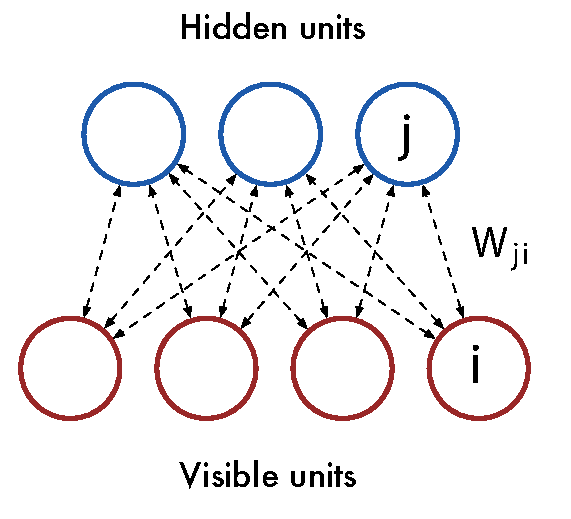
\includegraphics[scale=0.7]{RBM}
\caption{The \textit{Restricted Boltzmann Machine} (RBM) is defined by its units ($i$ or $j$) and weights ($W_{ij}$). Units are divided between visible units (4 units at the bottom) and hidden units (3 top-most). Weights and units define an energy function. Training an RBM consists in lowering the energy function around the example from a training set. Inference in this model is easy to perform since the hidden (resp. visible) units are independent from each others.}
\label{fig:RBM}
\end{figure}
An \textit{RBM} \cite{Hinton:2006:FLA:1161603.1161605} models the probability distribution of a set of random variables graphically represented as \textit{units}. Those units are divided between visible units, denoted by the vector $\bm{v} = (v_{1},...,v_{m})$, and hidden units, $\bm{h} = (h_{1},...,h_{n})$. In the simple model we present here, the visible units models the observed data and hence have the same dimensions, and hidden units some explanatory unobserved factors. The visible and hidden units are connected by weights $W_{ij}$. The joint probability of the visible and hidden units is given by $p_{model}(\bm{v},\bm{h}) = \frac{\exp^{-E(\bm{v},\bm{h})}}{Z}$ where
\begin{equation}
E(\bm{v},\bm{h}) = - \sum_{i=1}^{m} a_{i} v_{i}  - \sum_{i=1}^{m} \sum_{j=1}^{n} v_{i} W_{ij} h_{j} - \sum_{j = 1}^{n} b_{j} h_{j}
\end{equation}
is the energy function associated to the model and $Z = \sum_{v,h}\exp^{-E(v,h)}$ is the (usually intractable) partition function. $\bm{\theta} = \left\lbrace \bm{W} , \bm{a} , \bm{b} \right\rbrace$ is the set of parameters of the network.

In this context, training a model on a set of observed data means that we want the distribution of the model ($p_{model}$) to be as close as possible to the hypothetical real distribution of those data ($p_{data}$). A commonly used criterion is to maximize the likelihood of the training set, which can be defined as the probability those data have been sampled from the distribution of the model. The vector from the training set $\mathcal{D}$ are designated by $\bm{v^{(l)}}$.
Minimizing the negative log-likelihood is often preferred
\begin{equation}
\mathcal{L(\bm{\theta}|\mathcal{D})}  = \frac{1}{N_{\mathcal{D}}} \sum_{\bm{v^{(l)}} \in \mathcal{D}} - \ln \left[ p(\bm{v^{(l)}}|\bm{\theta})\right]
\end{equation}
where $N_{\mathcal{D}}$ is the size of the dataset. 

The search for the minimum of a non-linear function can be tackled by using gradient descent (REFERENCE). The gradient of the negative log-likelihood of a vector from the training database $\bm{v}^{(l)}$ is given by
\begin{equation}
- \frac{\partial \ln \left[ p(\bm{v^{(l)}}|\bm{\theta})\right]}{\partial \bm{\theta}} 
\approx 
\mathbb{E}_{p(\bm{h}|\bm{v^{(l)}})} \left[ \frac{\partial E(\bm{v^{(l)}},\bm{h})}{\partial \bm{\theta}} \right] 
- 
\mathbb{E}_{p(\bm{v} , \bm{h})} \left[ \frac{\partial E(\bm{v},\bm{h})}{\partial \bm{\theta}} \right]
\end{equation}
It is noteworthy to mention that it is formed by the difference between two expectation of the same quantity. The expectation on the left is often referred to as the \textit{data driven} term since it is an expectation over the distribution of the hidden units conditionally on a visible sample from the data distribution. 
The expectation on the right (minus sign) is referred to as the \textit{model driven} term since it is an expectation over the joint distribution of the model.
Unfortunately this quantity intractable because of the model driven term which involves a sum over all the possible configurations of the hidden (alternatively visible) units in order to compute the partition function (REF).

A training algorithm called \gls{CD} \cite{hinton2002training} rely on an approximation of the model driven term by running a k-step Gibbs chain to obtain a sample $\bm{v}^{(l,k)}$
\begin{equation}
\label{eq:grad_log_like}
- \frac{\partial \ln \left[ p(\bm{v^{(l)}}|\bm{\theta})\right]}{\partial \bm{\theta}}
\approx 
\mathbb{E}_{p(\bm{h}|\bm{v^{(l)}})} \left[ \frac{\partial E(\bm{v^{(l)}},\bm{h})}{\partial \bm{\theta}} \right] 
- 
\mathbb{E}_{p(\bm{h} | \bm{v^{(l,k)}})} \left[ \frac{\partial E(\bm{v^{(l,k)}},\bm{h})}{\partial \bm{\theta}} \right]
\end{equation}

Running a Gibbs sampling chain consists in alternatively sampling the hidden units knowing the visible units and the visible knowing the hidden \prettyref{eq:marginal_RBM}.
\begin{align}
\label{eq:marginal_RBM}
p(v_{i}=1|\bm{h}) &= \sigma \left( a_{i} + \sum_{j}W_{ij}h_{j} \right)\\
p(h_{j}=1|\bm{v}) &= \sigma \left( b_{j} + \sum_{i}W_{ij}v_{i} \right)
\end{align}
where $\sigma	(x) = \frac{1}{1+e^{-x}}$ is the \textit{sigmoid} function. Note that sampling from the marginal distribution is easy since visible units (respectively hidden units) are independent from each others. Hence, knowing the hidden units, all the visible units can be sampled in one step. This allows for a fast implementation of the samplings through matrix calculus, known as \textit{block sampling}.
It has been proved \cite{bengio2009learning} that the samples we obtain after an infinite number of iteration will be drawn from the joint distribution of the visible and hidden units of our model. Another approximation consists in starting the Gibbs chain from the sample $\bm{v}^{(l)}$, which increases the convergence of the chain, and limiting the number of sampling steps to a fixed number K. After evaluating the statistics for the distribution ($\bm{h} \sim p(\bm{h}|\bm{v^{(l)}})$ and $\bm{v^{(l,k)}}$ and $\bm{h}\sim p(\bm{h}|\bm{v^{(l)}})$ from the Gibbs sampling chain), the parameters can be updated. The whole algorithm is called Contrastive Divergence-K (CD-K). In a \textit{RBM} the update rules are given by
\begin{align}
\Delta W_{ij} &= <v_{i}h_{j} >_{data} - <v_{i}h_{j} >_{model}\\
\Delta a_{i} &= <v_{i}>_{data} - <v_{i}>_{model}\\
\Delta b_{j} &= <h_{j} >_{data} - <h_{j} >_{model}
\end{align}

\subsection{Conditional RBM}
\begin{figure}
\centering
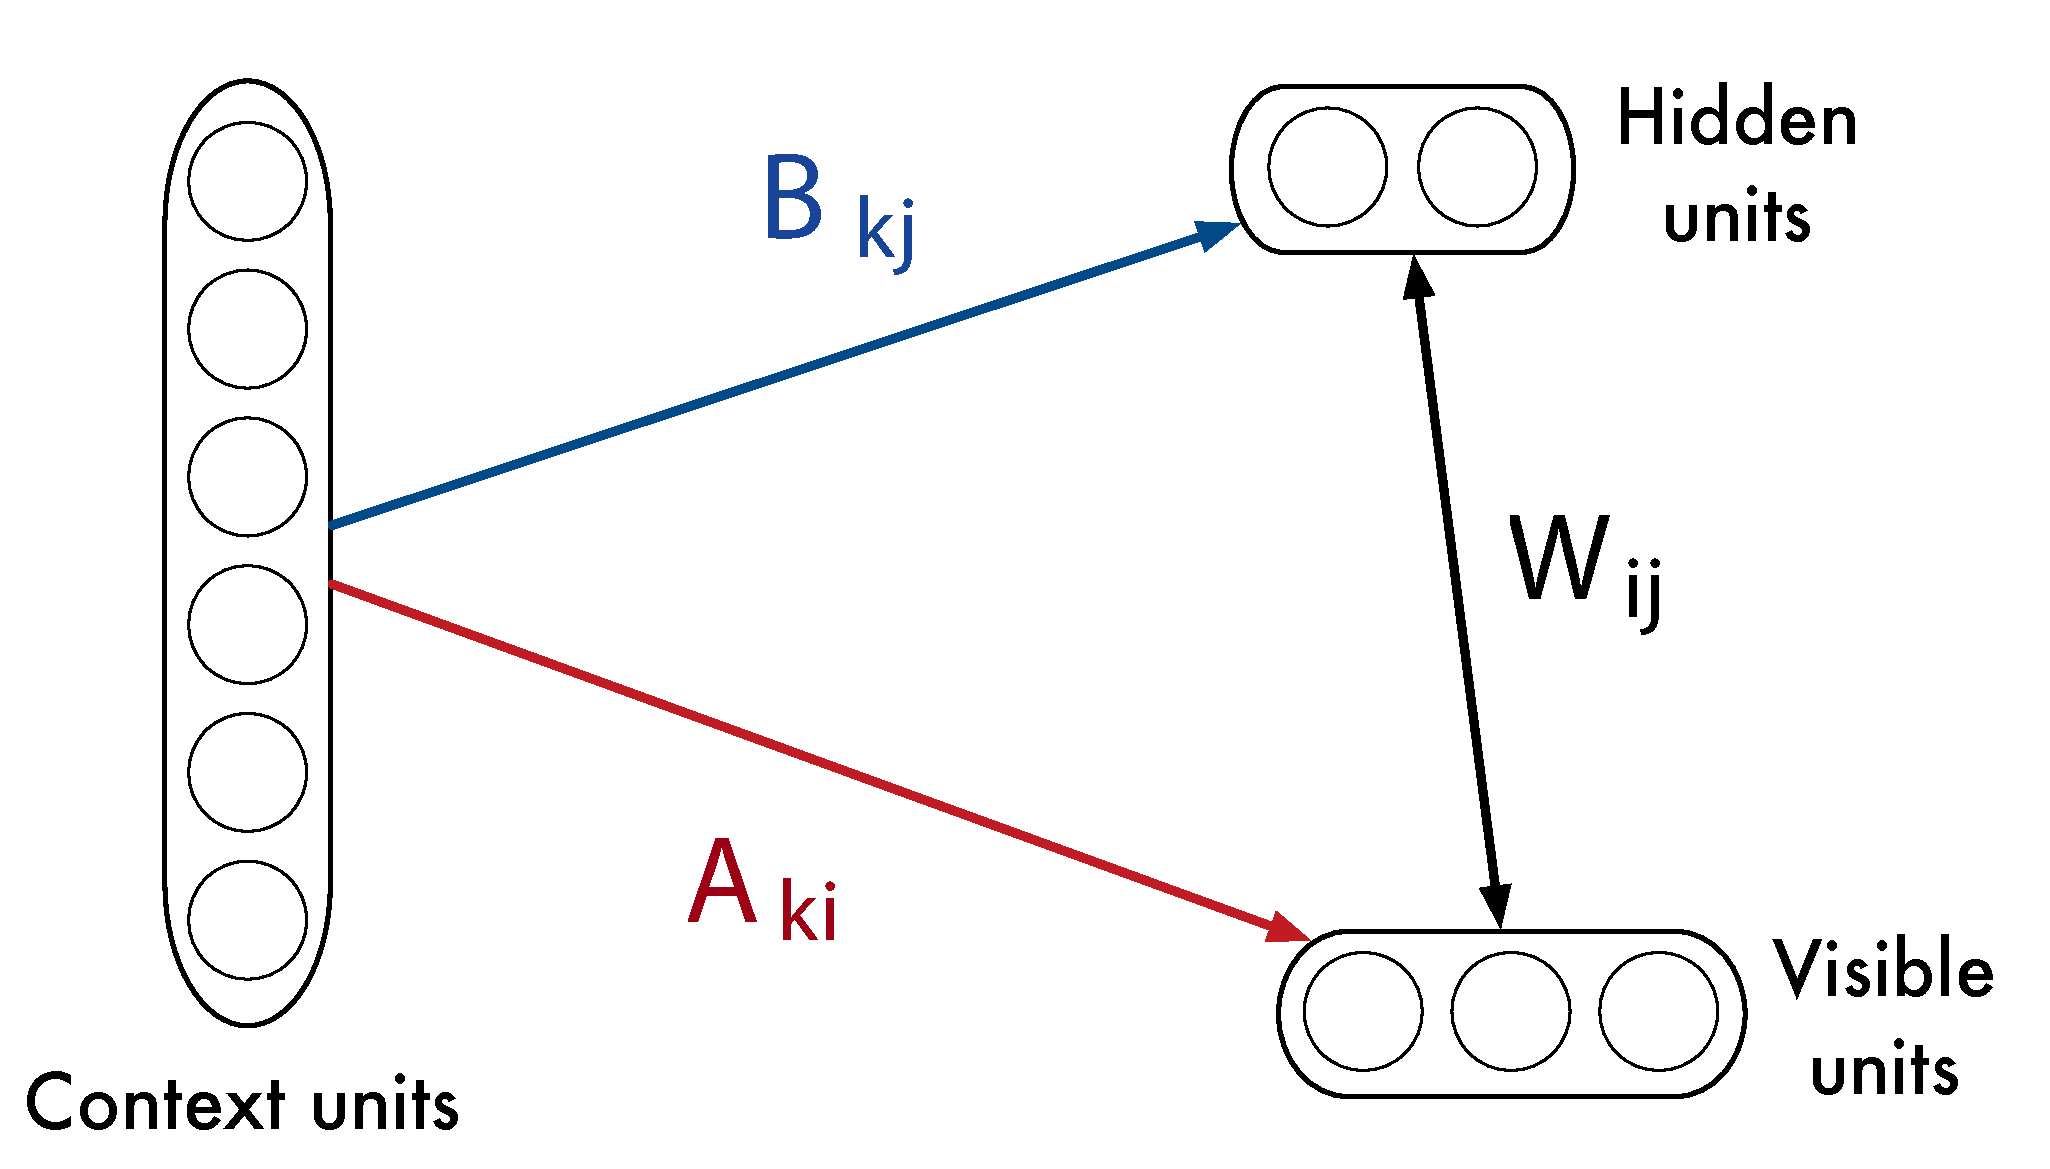
\includegraphics[scale=0.3]{CRBM_orchestration}
\caption{\textit{Conditional RBM} adds a layer of context units to the standard RBM architectures. Those context units linearly modify the bias of both visible and hidden units.}
\end{figure}
The Conditional \textit{RBM} model \cite{taylor2009composable} is an extension of the \gls{RBM} in which dynamic biases are added to the static biases of the visible and hidden units (respectively $\bm{a}$ and $\bm{b}$). This dynamic bias linearly depends on a set of units called context units $(\bm{x})$. Those context units can be used to represent the influence on the visible units of any other factor. Typically, when trying to model time series, those context units can be used to model the influence of the recent past frames over the current frame. Hence, if we now consider that the visible units are given for a certain time frame $\bm{v}(t)$, context units can be defined as the concatenation of the N last time frames $\bm{x}(t) = \left( v_{1}^{(t)} , ... , v_{m}^{(t)}, ... , v_{1}^{(t-N)} ... , v_{m}^{(t-N)} \right)$, where N denotes the temporal order of the model.
The energy function of the Conditional RBM is given by
\begin{equation}
\label{eq:energy_CRBM}
E(\bm{v}(t),\bm{h}(t)|\bm{x}(t)) = - \sum_{i} \hat{a}_{i}(t)v_{i}(t) - \sum_{ij}W_{ij}v_{i}(t)h_{j}(t) - \sum_{j} \hat{b}_{j}(t)h_{j}(t)
\end{equation}
where the biases are defined by 
\begin{align*}
\hat{a}_{i}(t) &= a_{i} + \sum_{k}A_{ki}x_{k}(t)\\
\hat{b}_{j}(t) &= b_{j} + \sum_{k}B_{kj}x_{k}(t)
\end{align*}
We will refer to the matrices $\bm{A}$ and $\bm{B}$ as \textit{auto-regressive matrices}.

This model can be trained using CD, since the marginal probabilities of visible and hidden units are the same as the \textit{RBM}, simply replacing the static biases by dynamics ones.
The following update rules are unchanged for $\bm{W}$, $\bm{a}$ and $\bm{b}$, and are the following for the auto-regressive matrices
\begin{align}
\Delta A_{ik} 	&=<v_{i}x_{k} >_{data} - <v_{i}x_{k} >_{model}\\
\Delta B_{jk} 	&= <h_{j}x_{k} >_{data} - <h_{j}x_{k} >_{model}\\
\end{align}

%\subsection{Factored Gated cRBM}
%\begin{figure}
%\centering
%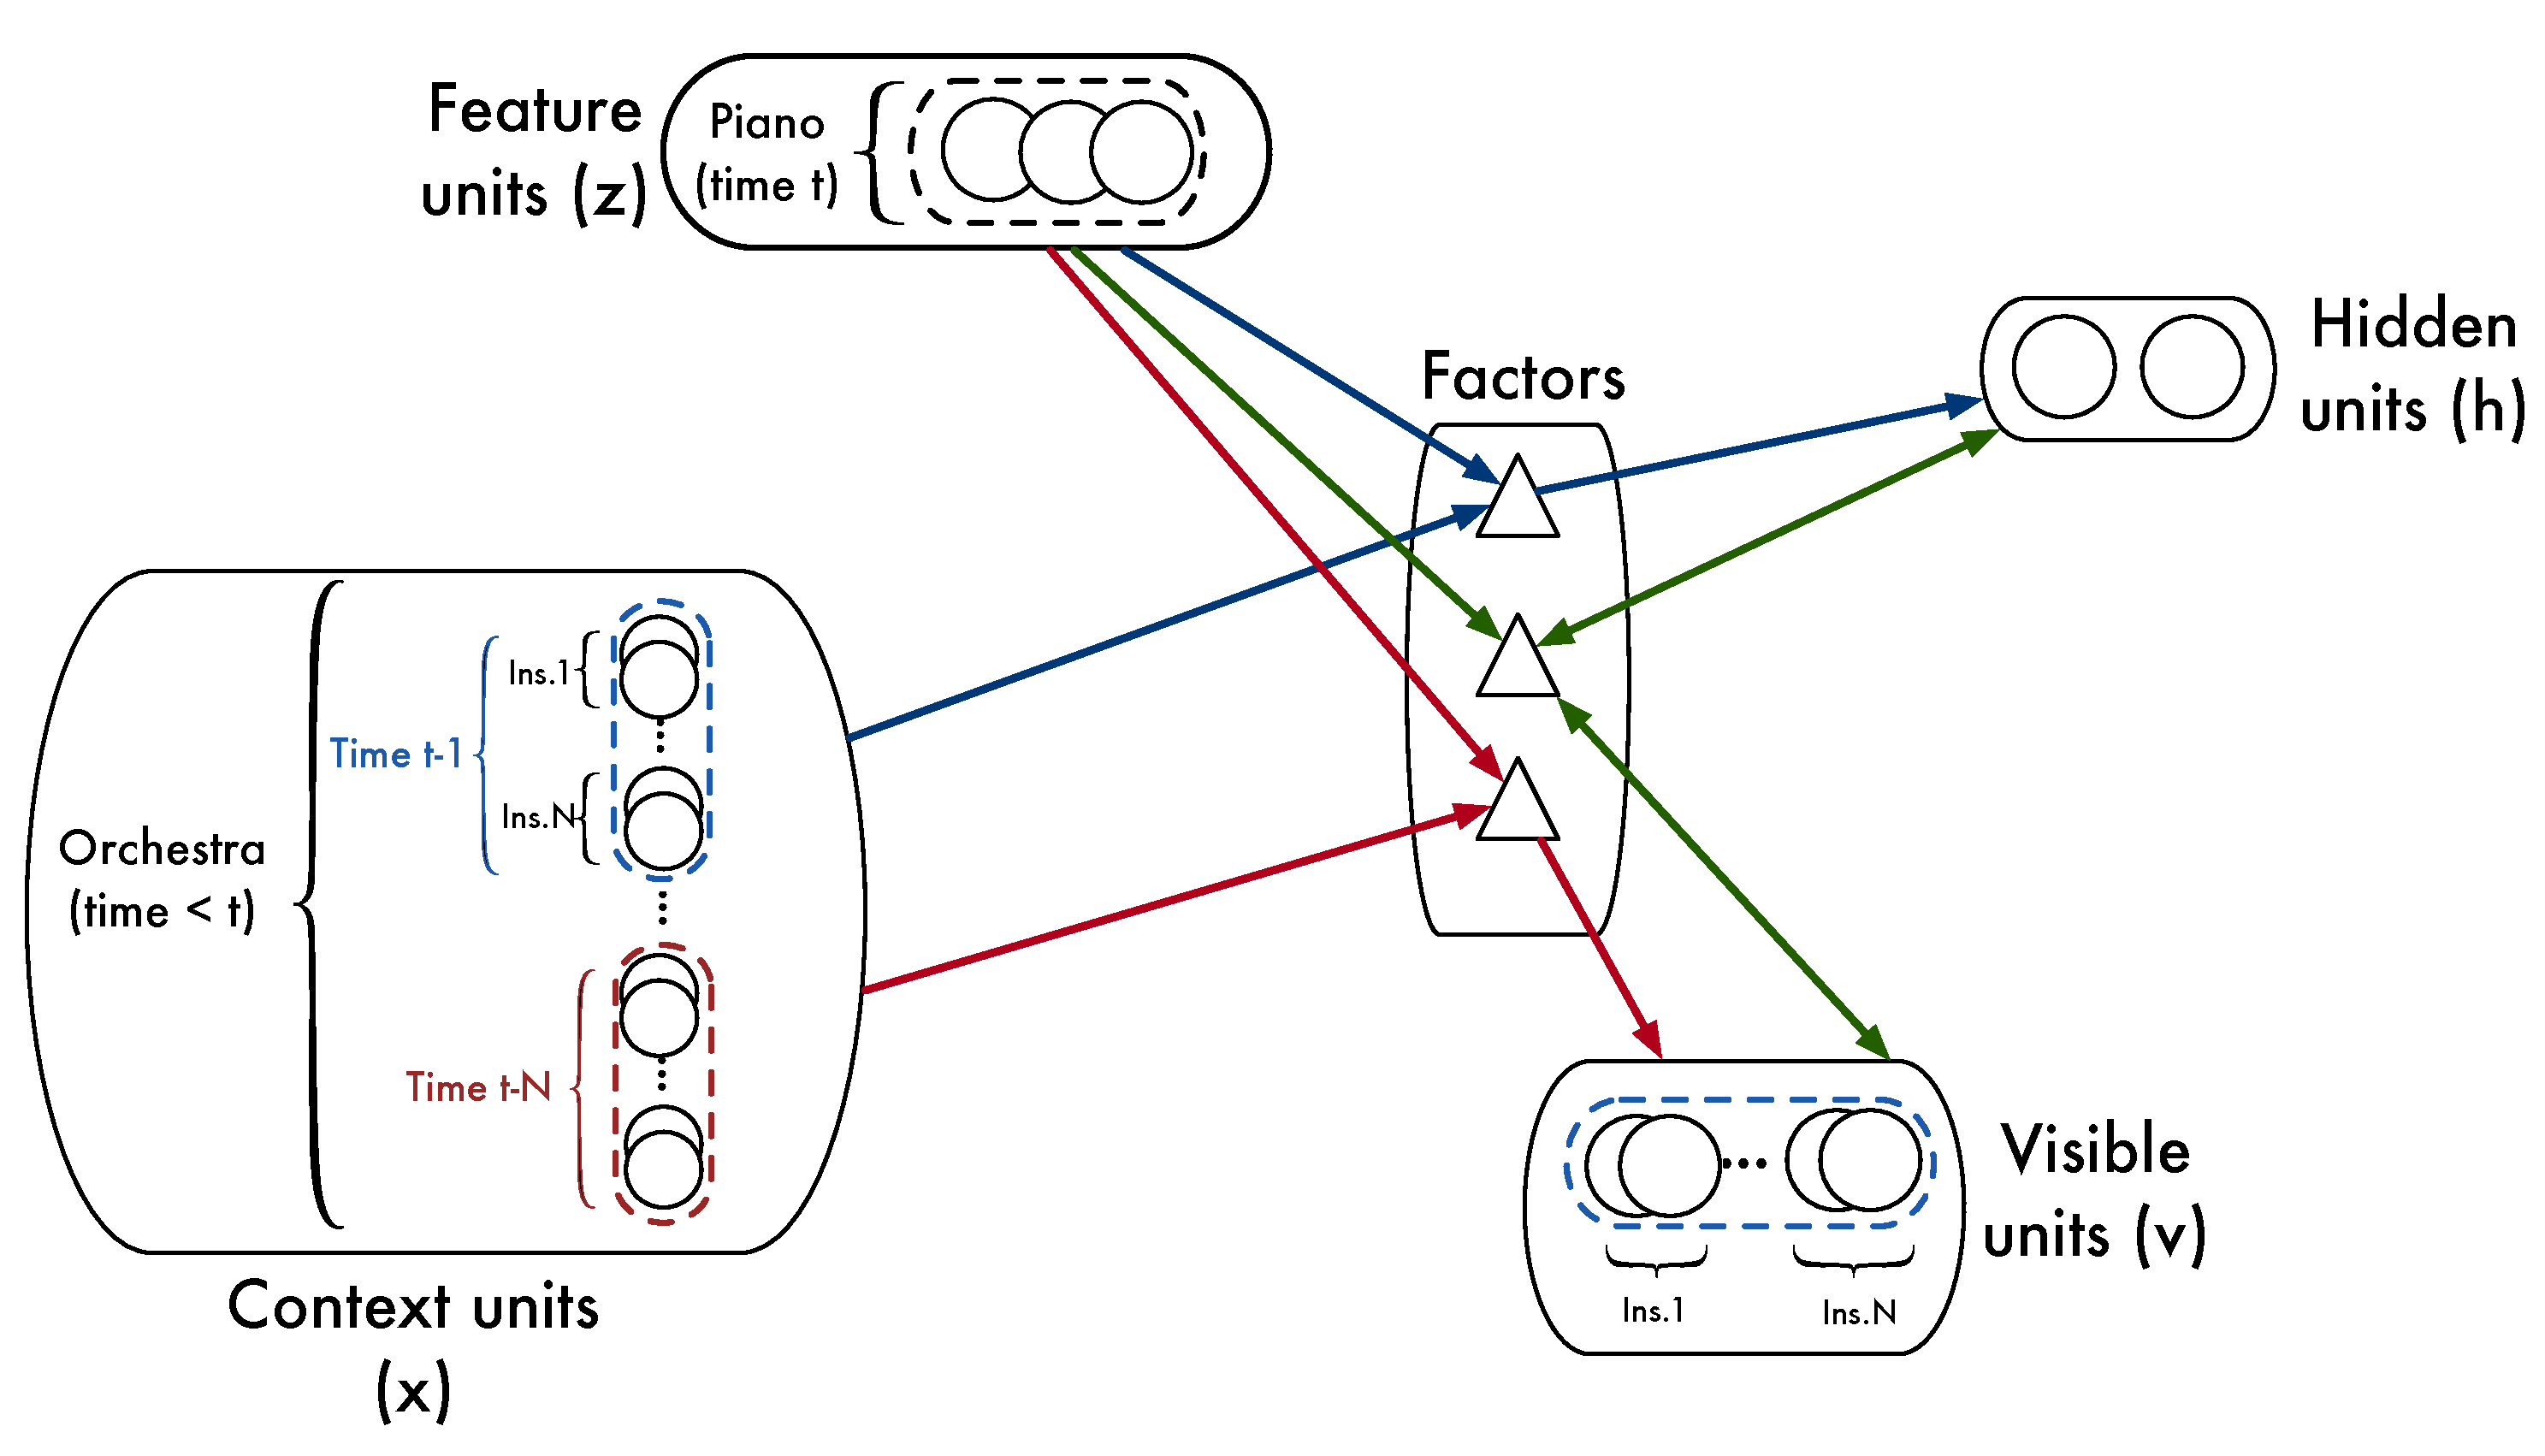
\includegraphics[scale=0.25]{FGCRBM_orchestration}
%\caption{\textit{FGCRBM} model. The features units ($\bm{z}$) modify the energy landscape of the model through a multiplicative influence over the weights $\bm{A}$, $\bm{B}$ and $\bm{W}$. Here, the role of each unit in the context of orchestration is indicated.}
%\label{fig:FGCRBM}
%\end{figure}
%The Factored Gated cRBM model (FGcRBM) \cite{taylor2009factored} proposes to extend the cRBM model by adding a layer of feature units $\bm{z}$ which modulate the weights of the conditional architecture in a multiplicative way. Hence, the parameters of the networks become $\bm{\theta} = \left\lbrace \bm{W} , \bm{A} , \bm{B} , \bm{a} , \bm{b} \right\rbrace$, where $\bm{W} = (W)_{ijl}$, $\bm{A}=(A)_{ikl}$ and $\bm{B}=(B)_{jkl}$ are three-dimensional tensors.
%
%This multiplicative influence can be interpreted as a modification of the energy function ($E$) of the model. Each configuration of the feature units defines a new energy function of the simple cRBM model defined by the other units ($\bm{v}$, $\bm{h}$, and $\bm{x}$). Since the number of parameters to train becomes high, the three dimensional tensors can be factorized into a product of three matrices by including factor units indexed by $f$ : $W_{ijl} = W_{if} . W_{jf} . W_{lf}$.
%The energy function of this Factored Gated Conditional RBM is then given by
%\begin{equation}
%E(\bm{v}(t),\bm{h}(t)|\bm{x}(t),\bm{z}(t)) = -\sum_{f}\sum_{ijl} W_{if}^{v} W_{jf}^{h} W_{lf}^{z} v_{i}(t) h_{j}(t) z_{l}(t) 
%- \sum_{i} \hat{a}_{i}(t)v_{i}(t) - \sum_{j} \hat{b}_{j}(t)h_{j}(t)
%\end{equation}
%where the dynamic biases of the visible and hidden units are defined by
%\begin{equation}
%\hat{a}_{i}(t) = a_{i} + \sum_{m} \sum_{kl}A_{im}^{v}A_{km}^{x}A_{lm}^{z}x_{k}(t)z_{l}(t)
%\end{equation}
%\begin{equation}
%\hat{b}_{j}(t) = b_{j} + \sum_{n} \sum_{kl}B_{jn}^{h}B_{kn}^{x}B_{ln}^{z}x_{k}(t)z_{l}(t)
%\end{equation}
%
%The \textit{FGCRBM} model can be trained by contrastive divergence which lead to the following update rules for the parameter
%\begin{align*}
%\Delta b_{i}^{(v)} &= <v_{i}>_{data} - <v_{i}>_{model}\\
%\Delta b_{j}^{(h)} &= <h_{j} >_{data} - <h_{j} >_{model}\\
%\Delta W_{if}^{v} &= <v_{i}\sum_{j} W_{jf} h_{j} \sum_{l} W_{lf} z_{l}>_{data} - <v_{i}W_{jf} h_{j} \sum_{l} W_{lf} z_{l} >_{model}\\
%\Delta W_{jf}^{h} &= <h_{j}\sum_{i}W_{if}v_{i} \sum_{l} W_{lf} z_{l}>_{data} - <h_{j}\sum_{i}W_{if}v_{i} \sum_{l} W_{lf} z_{l}>_{model}\\
%\Delta W_{lf}^{z} &= <z_{l}\sum_{i}W_{if}v_{i} \sum_{j} W_{jf}h_{j}>_{data} - <z_{l}\sum_{i}W_{if}v_{i} \sum_{j} W_{jf}h_{j}>_{model}\\\Delta A_{im}^{v} &= <v_{i}\sum_{k}A_{km}x_{k} \sum_{l}A_{lm}z_{l}>_{data} - <v_{i}\sum_{k}A_{km}x_{k} \sum_{l}A_{lm}z_{l}>_{model}\\
%\Delta A_{km}^{x} &= <x_{k}\sum_{i}A_{im}v_{i} \sum_{l}A_{lm}z_{l}>_{data} - <x_{k}\sum_{i}A_{im}v_{i} \sum_{l}A_{lm}z_{l}>_{model}\\
%\Delta A_{lm}^{z} &= <z_{l} \sum_{i}A_{im}v_{i} \sum_{k}A_{km}x_{k}>_{data} - <z_{l} \sum_{i}A_{im}v_{i} \sum_{k}A_{km}x_{k}>_{model}\\
%\Delta B_{jn}^{z} &=  <h_{j} \sum_{k}B_{kn}x_{k} \sum_{l}B_{ln}z_{l}>_{data} - <h_{j} \sum_{k}B_{kn}x_{k} \sum_{l}B_{ln}z_{l}>_{model}\\
%\Delta B_{kn}^{z} &= <x_{k} \sum_{j}B_{jn}h_{j} \sum_{l}B_{ln}z_{l}>_{data} - <x_{k} \sum_{j}B_{jn}h_{j} \sum_{l}B_{ln}z_{l}>_{model}\\
%\Delta B_{ln}^{z} &= <z_{l} \sum_{j}B_{jn}h_{j} \sum_{k}B_{kn}x_{k}>_{data} - <z_{l} \sum_{j}B_{jn}h_{j} \sum_{k}B_{kn}x_{k}>_{model}
%\end{align*}

\subsection{Generative models}
\begin{figure}
\centering
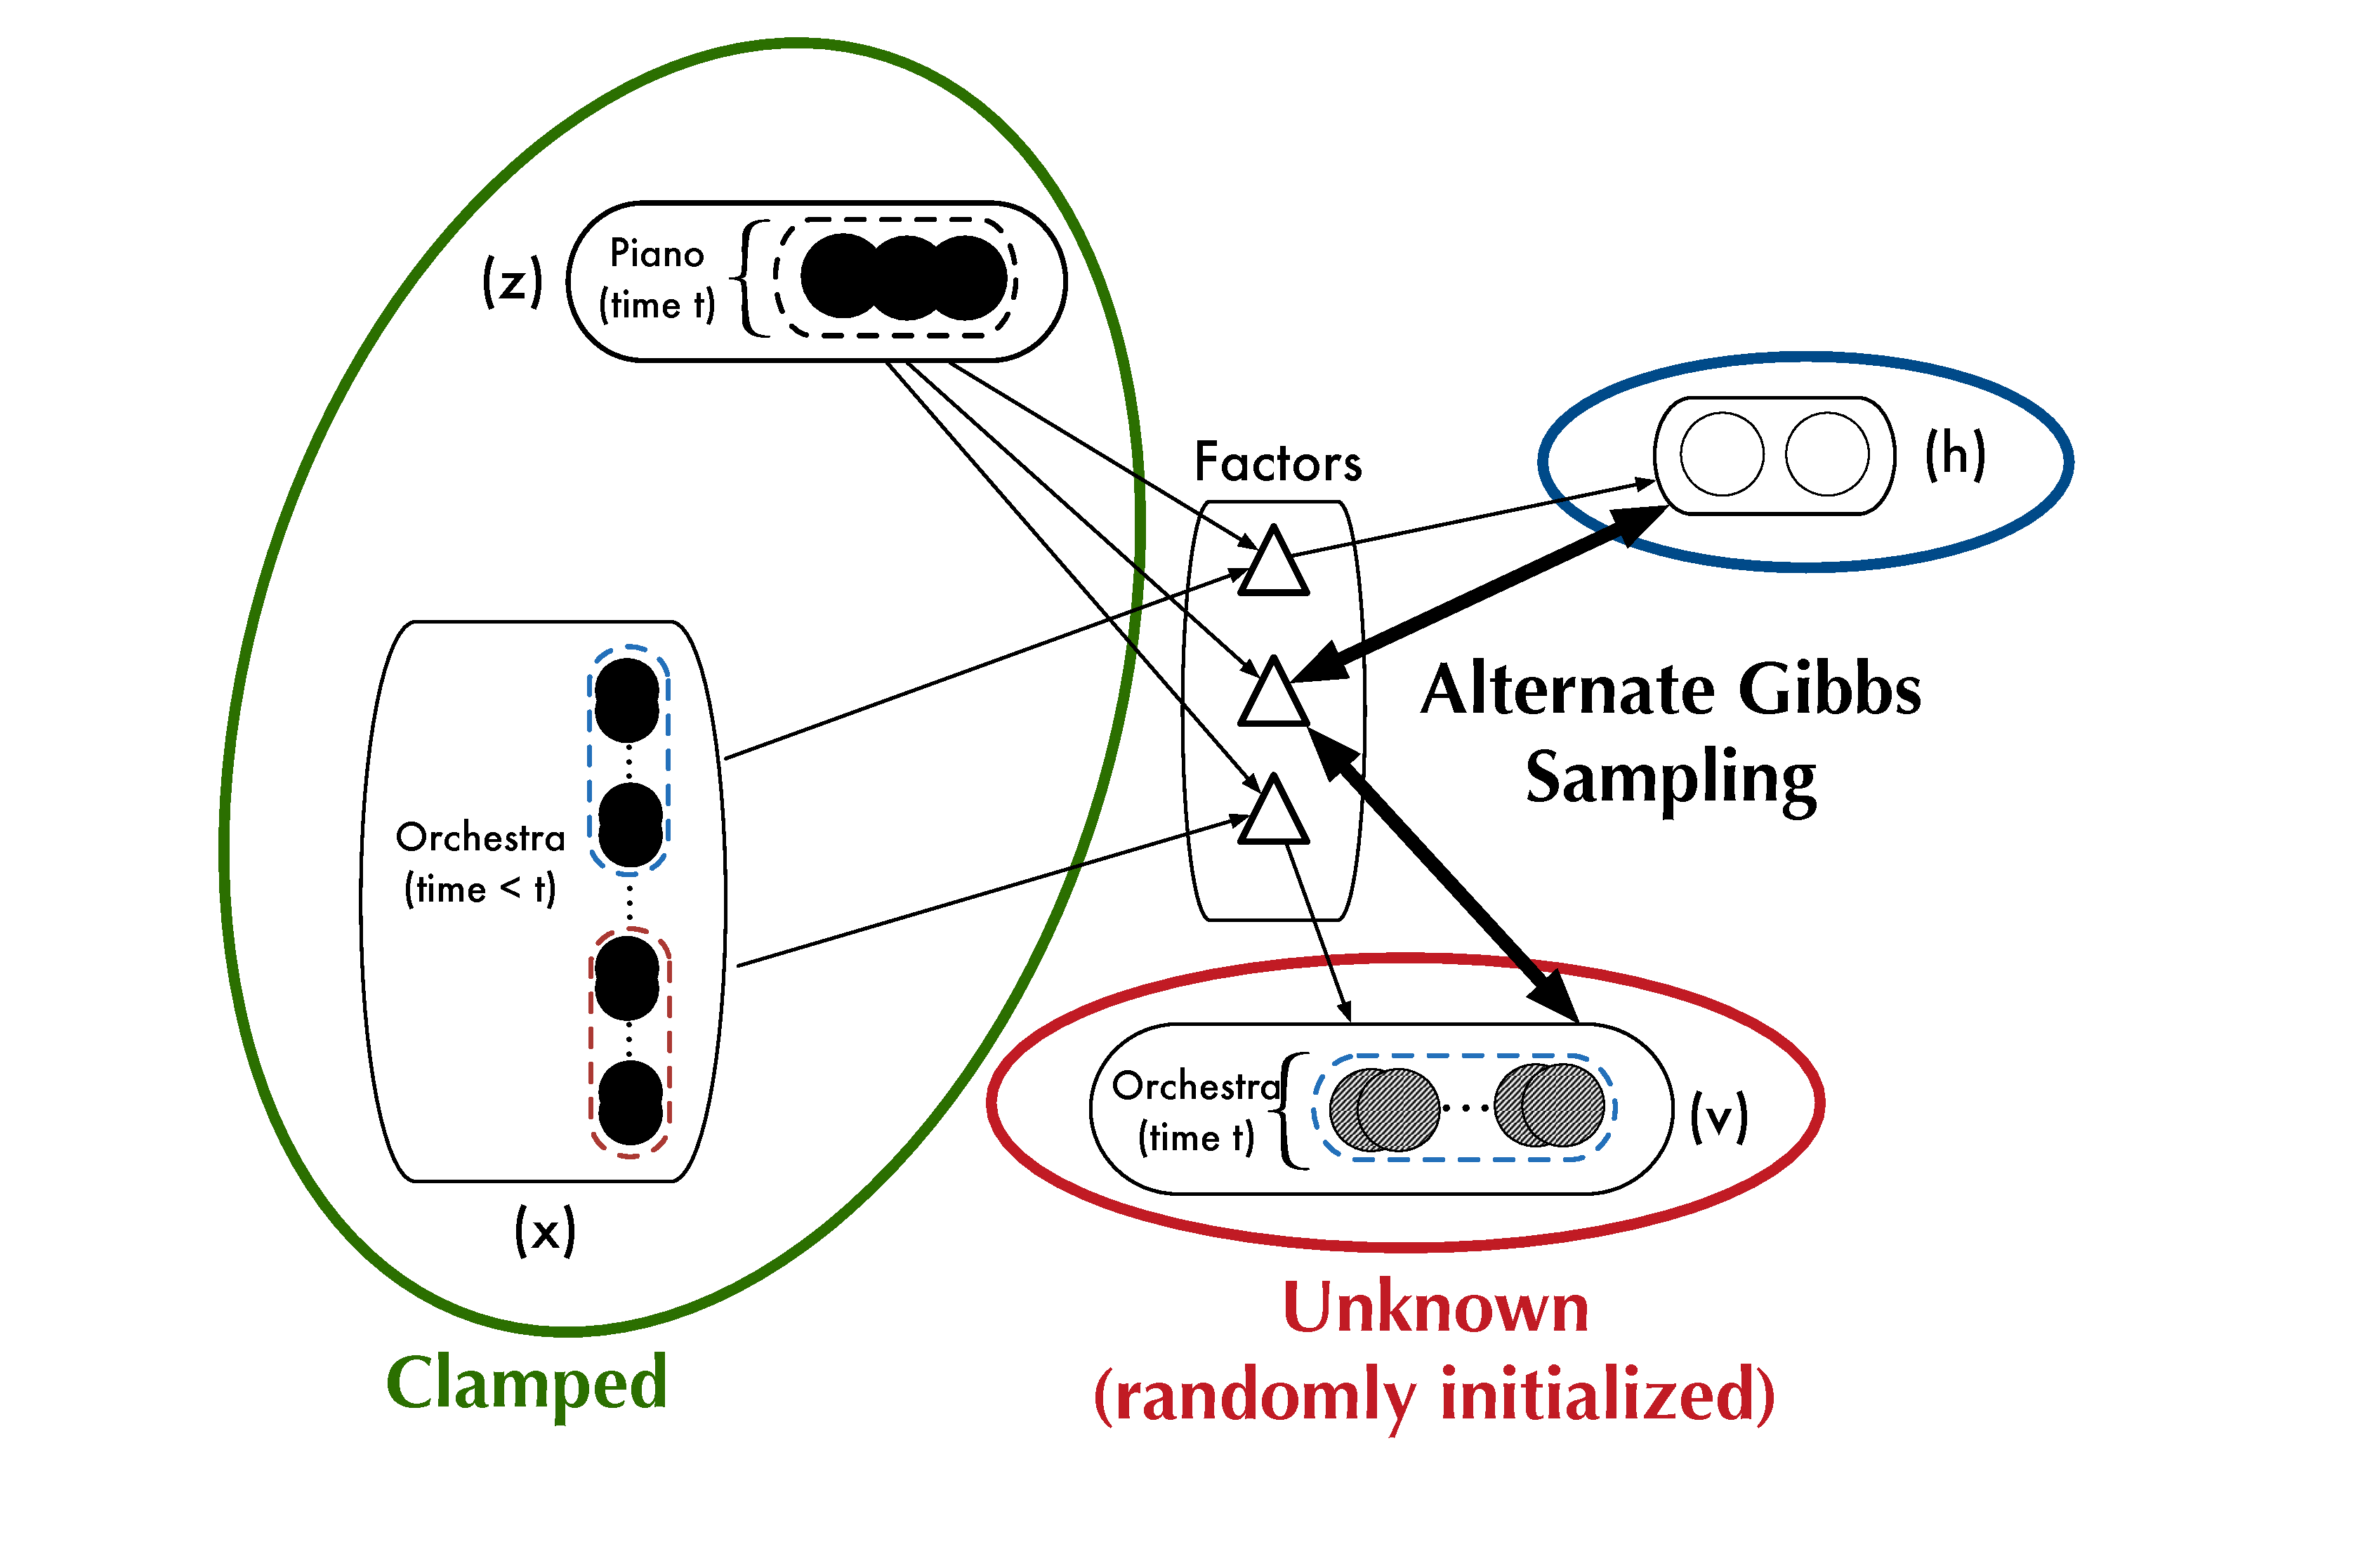
\includegraphics[scale=0.3]{FGCRBM_sampling}
\caption{\textit{Sampling in a FGCRBM}. Context and Features units are respectively clamped to the last ($t-1$ to $t-N$) orchestral frames and the current ($t$) piano frame. Visible units are randomly initialized. Then, several Gibbs sampling step are performed, in our case 40.}
\label{fig:FGCRBM_sampling}
\end{figure}
%% Role des unités conditionelles et tout le tralala dans les modèles
Once trained on a dataset using CD, those models represent a probability distribution $p$. If correctly trained, this distribution is supposed to be close (in the sense of the Kullback-Leibler divergence \cite{hinton2002training}) to the underlying probability distribution of the data. Then, by sampling from $p$, we are able to reproduce data \textit{similar} to the one observed in the training dataset.
This sampling process is called the generative step.

Sampling from \textit{RBM}-based models is not straightforward. 

Since the partition function is intractable, the marginal probability of the hidden and visible units cannot be sampled.
The generation process can be described as follow. After randomly setting the visible units vector (for each index $i$, $\bm{v}_{i} \sim \mathcal{U}(0,1)$), alternate Gibbs sampling is performed in order to approximate the joint distribution of the hidden and visible units conditionally on the context units. Given the context units, one step of alternate Gibbs sampling consists in sampling the hidden units knowing the visible, then sampling the visible units knowing the hidden. In theory the visible sample obtained is from the model distribution after an infinite number of steps. If theoretically an infinite number of steps is necessary, 20 to 100 steps are typically used in practice.

\subsection{Approximations}
In practice, several approximations are made both during the training and generative phases. The CD-K algorithm and its approximation, which consist in performing only a limited number of sampling steps and for the training phase starting the Gibbs chain with a sample from the training set, has already been discussed.

\subsubsection{Mean-field values} When evaluating the data and model-driven terms in equation \ref{eq:grad_log_like}, the two terms are the expectation of the same quantity under different distribution. For the data-driven term, this expectation is analytically derivable through the marginal probability of the hidden units, and ($\mathbb{E}\left[\bm{h}\right] = \sigma(\frac{1}{\bm{b} + \sum_{i} W_{ij}v_{i}})$).
For the model-driven term, expectation cannot be easily calculated since we do not have access to the joint probability. Approximating the expectation by running N Gibbs chains and computing an estimator would be too time consuming. Hence, a first idea is to "approximate" the expectation over $p(h|v^{(l,k)})$  by the value of the hidden vector obtained in the last step of the Gibbs chain ($\bm{h} \sim p(\bm{v^{(l,k)}})$).

Following the mathematical definition of an \textit{RBM}, the visible and hidden units must be sampled (thus equal to binaries values) from the marginal probabilities at each step of the Gibbs chain. However, it is possible to speed up the convergence of the algorithm by replacing the sampling value by the probability itself when updating the hidden vector at the last step k of the Gibbs chain : $\bm{h} = p(\bm{v^{(l,k)}})$. Doing this, we get rid of the sampling noise since the mean value of the marginal distribution is picked \cite{hinton2010practical}. Note that it is also possible to do so with the visible units at each time step, but it has been shown that it leads to a worse density estimation, which  is not a problem when the algorithm is used only as a pre-training step before 

\subsubsection{Number of sampling steps} It is interesting to note that $K=1$ in the CD-K algorithm during the training phase. This is because the objective is to modify the energy of our model in order to increase the likelihood  of the training set under the model distribution. It has been shown that even a small number of sampling steps guarantees to increase a lower bound over the likelihood \cite{bengio2009learning}. When generating data, we seek to obtain a sample from the distribution of the model. Therefore, a larger number of Gibbs sampling steps need to be performed in order to effectively obtain a good approximation.

\section{Projective orchestration}
In this section, we present how to perform automatic projective orchestration using a cRBM. In particular, we detail which kind of data representation we used and the modelling function of the different units.
A objective criterion of the performances of a model is necessary. Not only to compare the different systems, but also to find the best set of hyper-parameter for a given model. To our best knowledge, there is no quantitative evaluation framework for automatic projective orchestration. We propose here a first attempt in order to fill this gap by defining a projective orchestration inference task. Given a test database composed by piano scores and orchestrations proposed by experts (famous composer), it consists at each time frame $t$ to generate an orchestral vector $\hat{Orch}(t)$ knowing the piano frame $Piano(t)$ and the recent past of sequence of orchestral vectors $Orch(t-1),... Orch(t-N)$. The predicted vector $\hat{Orch}(t)$ is then compared to the ground-truth $Orch(t)$ via an accuracy measure.
The database used and results obtained with the \textit{cRBM} are then presented in the two last sections.

\subsection{Formalization}
Conditional models allow to generate sequences of data under a certain context. Projective orchestration can be seen as producing an orchestral score, conditionally on a piano score. In order to guarantee a form of temporal continuity in the orchestration, the recent past of the orchestral sequence is added in the contextual information.

\subsubsection{Data representation}
\label{sec:data_representation}
Before being able to train the previously introduced models, the first step is to choose an adapted representation for the piano and orchestra information.
\begin{figure}
\centering
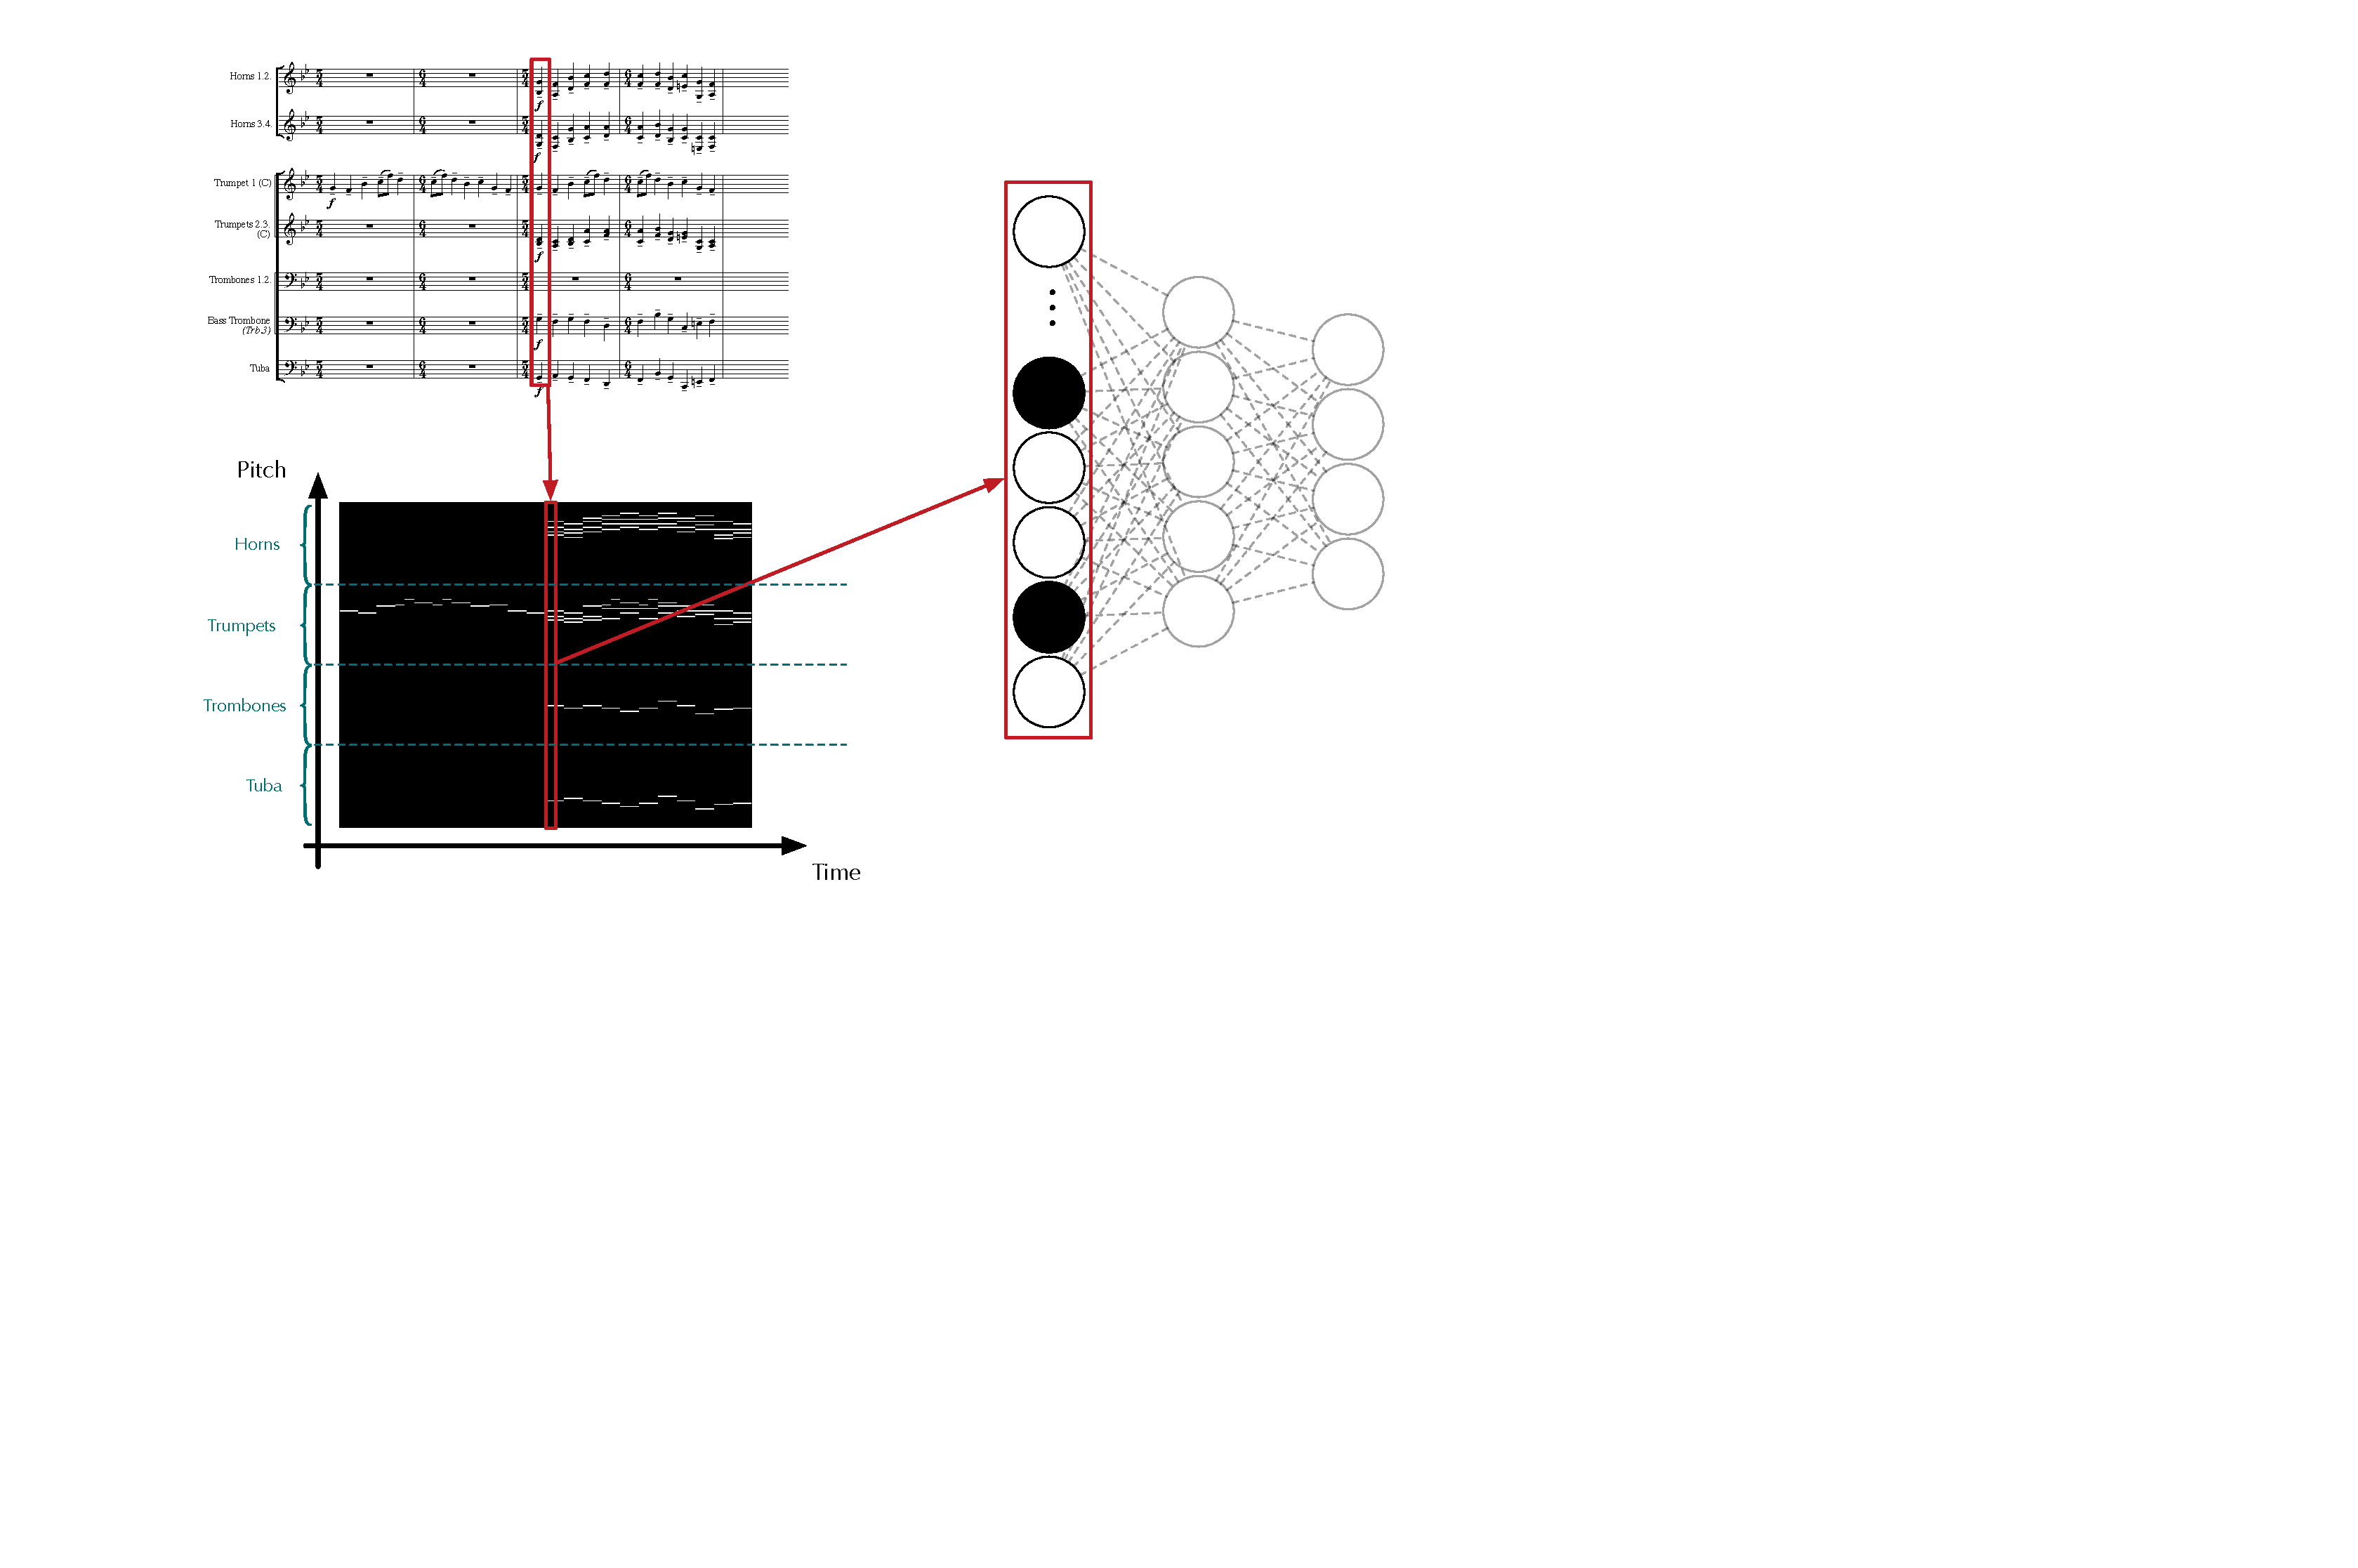
\includegraphics[scale=0.55]{data_representation}
\caption{The successive visible units of a neural network could be the successive temporal frames of a \textit{pianoroll}. A \textit{pianoroll} is a representation of musical events, discrete on both the frequency (pitch) and the time (frames) scales. For a single instrument, a pitch $p$ at time $t$ can be either played or not, which is represented by a one or zero in the \textit{pianoroll}. This definition is extended to an orchestra by simply concatenating the \textit{pianorolls} of each instruments along the pitch dimension. One can see on the figure that the same instruments are grouped together event if they don't play the same thing. For instance, trumpets 1, 2, 3 and 4 are grouped under one trumpet part, which then contains 4 voices chords.}
\label{fig:pianoroll}
\end{figure}
The \textit{pianoroll} representation is often used to model sequences of symbolic music.
this is a binary matrix $Pianoroll(p,t)$ of dimension $N_{T} \times N_{P}$.
For a single instrument $N_{T}$ is the temporal length of the musical sequence,  and $N_{P}$ the number of pitches potentially played by the instrument. Hence, for a certain time quantisation $Pianoroll(p,t)$ specifies if a pitch $p$ is played at time frame $t$.
The dynamics are ignored and each time frame can be represented by a binary vector $Pianoroll(t) \in \left\lbrace 0  1 \right\rbrace ^{N_{P}}$.
As depicted in figure \ref{fig:pianoroll}, this representation can be easily extended to an orchestra composed by $N_{I}$ instruments by simply concatenating the \textit{pianorolls} of each instrument over the pitch dimension.

In the proposed system, two different \textit{pianorolls} are used to represent the piano and the orchestra score.
For the piano score, $N_{P} = 88$ since this is the number of keys for a standard grand piano.
The orchestra representation require more attention. Each instrument has a different playing range. Hence, the size of their pitch dimension is different for each. In practice, we limited it to the pitch observed in the training dataset. The observed range is denoted $R(i)$ for each instrument $i$ in an set of instrument $I = {\text{violin},\text{viola},...}$. If the training base is sufficiently large, every note that can be played by each instrument will be seen at least once. This restriction acts as an important constraint over the playing range of each instrument by preventing the system to assign absurd notes to the different instrument (for instance a low register note to a piccolo).

Note that we follow the usual orchestral simplifications used when writing orchestral scores by grouping together all the instruments of a same section. For instance, the section \textit{violin 1}, composed by many instrumentalists (10 or more), is written as a single part.
Eventually, following the notations we just introduced, the dimension of an orchestra \textit{pianoroll} composed by the instrument set $I$ are given by $N_{T} \times \sum_{i \in I} R(i)$.

In our framework we chose 14 instruments indexed by 
\begin{figure}
\begin{center}
\begin{tabular}{|r|r|c|r|r|}
\cline{1-2}
\cline{4-5}
\rule{0pt}{2.5ex} Index & Instrument & & Index & Instrument\\
\cline{1-2}
\cline{4-5}
\rule{0pt}{2.5ex} 1 & Violin & & 8 & Trombone\\
2 & Viola & & 9 & Tuba\\
3 & Cello &  & 10 & French horn\\
4 & Double-bass & & 11 & Oboe\\
5 & Harp & & 12 & Bassoon\\
6 & Timpani & & 13 & Clarinet\\
7 & Trumpet & & 14 & Flute\\
\cline{1-2}
\cline{4-5}
\end{tabular}
\end{center}
\caption{Indexation used for the orchestra instruments}
\end{figure}

\subsubsection{Modeling orchestral sequences}
For a piece of music, we define two sequences of vectors $Orch(t)$ and $Piano(t)$ with $t$ in $\left[ | 1 , N_{T} | \right]$ where $N_{T}$ is the lenght of the piece. Those are respectively defined by the sequence of column vector from the \textit{pianoroll} representation of the orchestra part and of the piano part.

At each time frame $t$, the visible units of the cRBM represent the current orchestral vector ($Orch(t)$), conditional units are used to model the influence of the past orchestral vectors $Orch(t-1) , ... , Orch(t-N)$ and the influence of the current piano frame ($Piano(t)$) over the visible units. The context units are then defined by the concatenation of the past orchestral frames and the current piano frame
$ Context(t) = \left[ Piano(t) , Orch(t-1) , ... , Orch(t-N)\right]$.

%The \textit{FGCRBM} model allows to separate the influence of the current piano frame and the past orchestral frames. The current piano frame defines the feature units ($z$) $ Features(t) = Piano(t)^{T} $, and the concatenation of the past orchestral frames define the context units ($x$) $ Context(t) = \left[ Orch(t-1)^{T} , ... , Orch(t-N)^{T} \right]^{T}$ (\prettyref{fig:FGCRBM}).

Note that we do not restrain the possible pitches of each instrument to the pitches seen in the piano score at each specific time frame. Indeed, orchestrating a piano score cannot be reduced to the simple repartition between the different instruments of the same notes already written in the piano score. Instead, the harmonic structure is often enriched by extra notes, ranging from simple octaviations to harmonic expansions (more complex chords with a specific colour). The melody might be doubled by several instruments at the unison, octave or even double octave.
+ Something about the phrasing ? A wind instru can't play the same phrasing as a pianist. Reciprocally, a pianist can't tremolo

\subsection{Evaluation}
Building a quantitative evaluation framework for generative models is rarely straightforward, especially since computing the likelihood of a test sample is intractable in the models we used. A common practice is to define an auxiliary task close to the generative objective but easier to evaluate.
Typically, in automatic music generation, the models are evaluated through a predictive task based on a frame-level accuracy measure \cite{DBLP:journals/corr/LiuR14a,boulanger2012modeling,lavrenko2003polyphonic}. We introduce an extension of this evaluation framework to an orchestral context through a task called \textit{frame-level orchestral inference}. This framework heavily relies on the previous works in automatic music generation and we discovered a bias in the measurement due to the temporal scale used (frame-level). We then propose a new evaluation framework and present the results of our system in a newly introduced \textit{event-level} framework.

\subsubsection{Frame-level accuracy}
The frame-level accuracy of a model is defined as the mean value of the accuracies measured for each time frame of a testing set.
For each time frame, we try to predict the orchestral frame $\hat{Orch}(t)$ knowing the recent past $Orch(t-1),...,Orch(t-N)$ and the piano frame $Piano(t)$ and compare it to the original frame $Orch(t)$. The accuracy measure the difference between the predicted and original frames \cite{boulanger2012modeling,DBLP:journals/corr/LiuR14a}
\begin{equation}
\text{Accuracy}  = \frac{TP(t)}{TP(t) + FP(t) + FN(t)}
\label{eq:accuracy}
\end{equation}
where $TP(t)$ is the number of notes correctly predicted (true positives). $FP(t)$ is the number of notes predicted which are not in the original sequence (false positive) and $FN(t)$ is the number on unreported notes (false negative). 

Instead of binary values, activation probabilities are used for the predicted samples in order to reduce the sampling noise. In the case this probability is intractable, one should sample many predicted frames for each time frame and compute the mean value of those samples.

\subsubsection{Event-level accuracy}
A major flaw in the frame-level accuracy measure is its dependence to the rhythmic quantization chosen. Indeed, when the quantization become too small, it becomes highly probable that a frame is simply repeated at the next time frame. Hence, the best predictive model is simply a model which predict that the next time frame is the same as the frame $t-1$. This is not a desirable behaviour, and we propose an evaluation based on an event-level to address that issue.

A musical event is defined as a change in the orchestral score, either a note being switched on or off. The predictive event-level accuracy measure relies on the same accuracy measure previously defined \prettyref{eq:accuracy}. The only difference is that it occurs at each new event instead of each new time frame. Since the task is slightly different, the training phase has been consequently changed so that a model is trained only on new event frames.

% Be careful, event level not on the context

\subsection{Database}
We used a parallel database of piano scores and their orchestration by famous composers. The database consists of 76 \textit{XML} files. Given the complexity of the distribution we wanted to model and the reduced size of the database we have accessed to, we decided to keep as a test dataset only the last half of one track from our database. Hence 75 and a half files were used to train our model. We chose to do so in order to have the best generation ability.
The contrastive-divergence algorithm has been applied on mini-batches of size $100$ during the training phase. Thus we obtained $335$ mini-batches for the frame-level measure, and $89$ for the event-level measure.
For each instrument, the pitch range is reduced to the \textit{tessitura} observed in the training dataset (\label{sec:data_representation}). We used a rhythmic quantization of 8 frames per beat.

\subsection{Results}
We evaluated the \textit{CRBM} and \textit{FGCRBM} previously presented \prettyref{sec:state_of_the_art} in both the frame-level and event-level frameworks. Those two models are compared to a random prediction of each frame and to a simple model that outputs the previous frame as the current frame prediction (i.e. a untrained 1 order linear predictor). The results are presented in the following tables \prettyref{fig:result_frame} and \prettyref{fig:result_event}.

% Frame
% Event
%
% Precision et accuracy
%
% Séparer repeat et change true/false positive

\begin{figure}
\centering
\begin{tabular}{c c}
\hline
\multirow{2}{*}{Model} & Orchestral Frame-level (\%)\\
\hline
Random & 0.51\\ 
Repeat & 93.25\\ 
\hline \hline
CRBM & 45.07\\ 
FGCRBM & 2.05\\ 
\end{tabular}
\caption{Frame-level accuracy}
\label{fig:result_frame}
\end{figure}

\begin{figure}
\centering
\begin{tabular}{c c}
\hline
\multirow{2}{*}{Model} & Orchestral Event-level (\%)\\
\hline
Random & 0.50\\ 
Repeat & 93.25\\ 
\hline \hline
CRBM & 27.78\\ 
FGCRBM & \\ 
\end{tabular}
\caption{Event-level accuracy}
\label{fig:result_frame}
\end{figure}
%% C'est de la merde, même le edvent-level ça règle pas du tout le problème : soit on prédit l'event mais avec un context basé sur les frames, et dans ce cas là le modèle repeat est bon, soit on prends que les event mais ça n'a aucun sens (pas de rythme...)

\section{Live Orchestral Piano}


\section{Conclusion and future works}
% Better DB
% Change the data representation

% Acknowledgments
\begin{acks}
The authors would like to thank
\end{acks}

% Bibliography
\bibliographystyle{ACM-Reference-Format-Journals}
\bibliography{biblio}
                             % Sample .bib file with references that match those in
                             % the 'Specifications Document (V1.5)' as well containing
                             % 'legacy' bibs and bibs with 'alternate codings'.
                             % Gerry Murray - March 2012

\medskip

\end{document}
% End of v2-acmsmall-sample.tex (March 2012) - Gerry Murray, ACM
